\documentclass[../main.tex]{subfiles}

\begin{document}

The Tangle is a data structure built in accordance with the following rule:

\begin{displayquote}
    \textit{In order to join the Tangle, a transaction has to validate two existing transactions.}
\end{displayquote}

\noindent
The validation of a transaction is a procedure that verifies whether an address owns the tokens spent\footnote{The actual validation process in IOTA is more complex, and we invite the interested reader to visit \url{https://docs.iota.org} for more information.}. If transaction $y$ validates transaction $x$, we say that $y$ \textit{directly} approves $x$. Conversely, if there is not a directed edge between the transactions $x$ and $y$, but there exists a directed path between them, then we say that $y$ \textit{indirectly} approves $x$.

The IOTA white paper originally uses only a TSA based on a biased random walk to determine the tips to approve. This TSA has a double benefit: First, it is effective against selfish nodes that do simple selections (e.g., at random or at the genesis) to avoid the effort of tip selection; second, it makes the Tangle more resistant against malicious nodes performing, e.g., parasite chain attacks (see Fig.~\ref{fig:parasite_chain}). However, the white paper proposal comes with its own limitations as discussed in Section~\ref{sec:cliri}; in particular, an honest transaction majority is a necessary condition for the security of the algorithm.

\begin{figure}[htb]
     \centering
     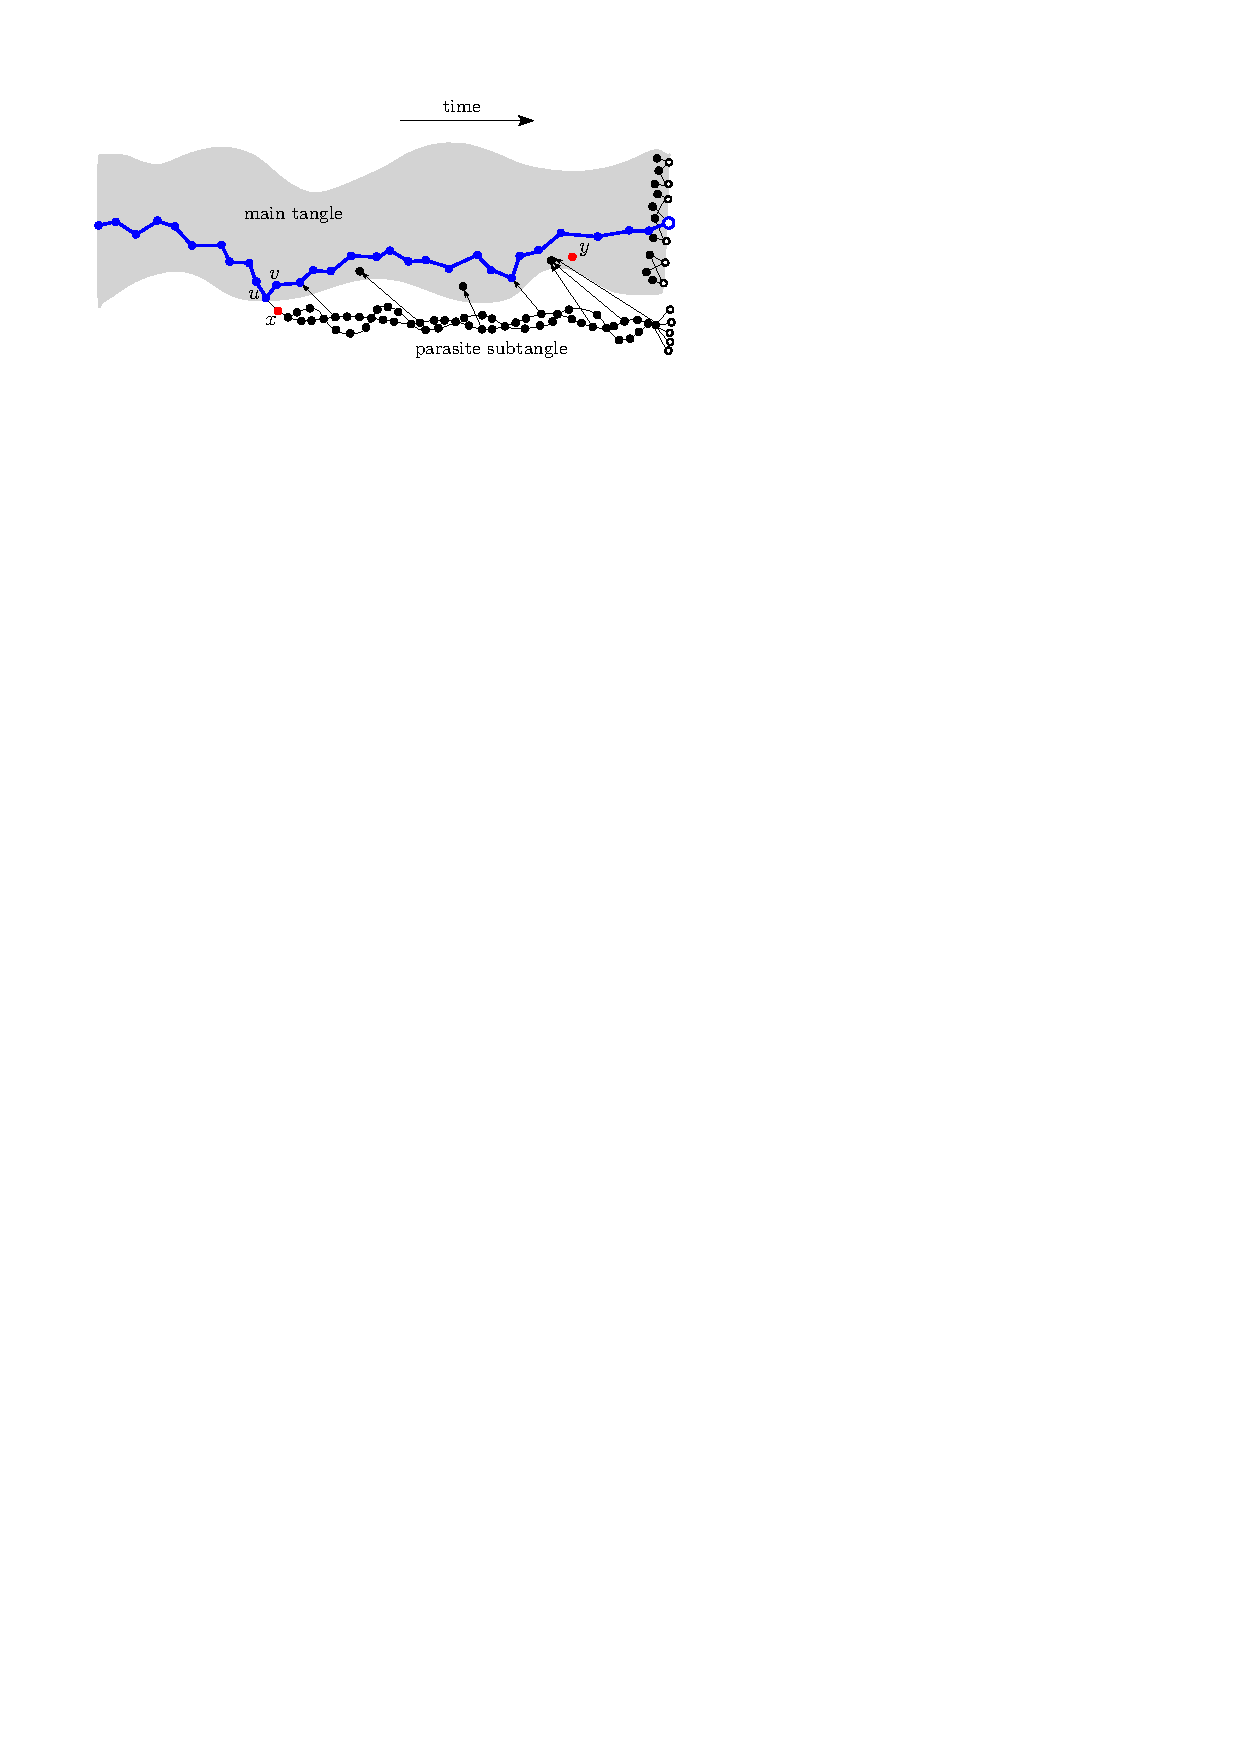
\includegraphics[width=0.75\textwidth]{images/par_attack.pdf}
     \caption{An illustration of the parasite chain attack: The transaction $x$ spends the funds that the attacker wants to spend once more in transaction $y$, before revealing the subtangle containing $x$. The grey area contains many transactions which are not shown for sake of clarity. The thick blue line corresponds to a trajectory of a typical random walk.}
     \label{fig:parasite_chain}
\end{figure}

In the rest of this section, we provide an overview of the current status of the research on TSAs:
Specifically, in Section~\ref{sec:tsa_rw} we introduce a random walk-based TSA which aims to improve the original white paper algorithm;
then, in Section~\ref{sec:tsa_non-rw} we investigate an alternative approach where two different algorithms are used to choose each one of the two tips to approve.

It is important to stress that, since the TSA is not (and cannot be) enforced, the choice of the particular TSA is, \emph{ultimately}, up to the node's owner. Therefore, the actors will choose their TSAs in a \emph{reasonable} way, as argued in~\cite{popov2019feelessfree}.  Because of this intrinsic freedom of choice, and also because the ``space'' of all possible TSAs is enormous, it is crucial to have all reasonable options on the table. We are absolutely not obliged to be ever content with a particular version of TSA; instead, our vision is that, similarly to the human society itself, the system will continue evolving. Therefore, although the existing random walk-based TSAs are already doing a good job, we will describe below several over promising  options and research directions, which would hopefully invite the academic community to provide more valuable input.

\subsubsection{Random walk-based TSA}\label{sec:tsa_rw}

The TSA of the white paper is a biased random walk that starts from the genesis transaction and walks towards the tips. Once the walk has reached a tip, that tip is chosen as the first direct approvee. A second walk is then performed to choose the second direct approvee. In order to prevent the random walk from ``lazy'' tips choosing to validate old transactions, the transition probability from transaction $x$ to transaction $y$ is biased and proportional to
\begin{equation}\label{eq:transition_prob}
    \mathbf{P}[x\rightarrow y] \propto \exp\left\{\alpha\cdot w_y\right\},
\end{equation}
where $\alpha>0$ is a weight parameter, and $w_y$ is the cumulative weight\footnote{The definition of cumulative weight in the white paper is slightly more general and also considers the work needed to issue transactions.}, i.e., the number of transactions that directly or indirectly approves $y$. In order to obtain the actual probability, one can simply normalize Eq.~\eqref{eq:transition_prob}. Since every node sees a different set of tips, it is thus not possible to impose a given TSA.

In this section, we provide an alternative random walk-based algorithm to improve security and performance. As already specified in the text, although the TSA cannot be enforced, we expect that a node would follow the ``best'' algorithm available. The main idea is to introduce a local (i.e., per-node) view of the Tangle such that some transactions are preferred based on various kinds of information locally available at the nodes. For instance, the time of solidification\footnote{The time of solidification of transaction $x$ is the time at which not only the transaction itself, but also all transactions referenced by $x$ have been received by a given node.} could be used to reduce the effectiveness of parasite chain attacks:
Since an attacker would require some time to build a subtangle, an honest node could decide to penalize a transaction that appears later than it should. Such a local view is commonly called \textit{local modifiers}~\cite{popov2018lm}.

In general, local modifiers enable multiple features: They strengthen the security of the Tangle, especially against parasite chain and splitting attacks; they reduce the dependency on PoW and the cumulative weight calculations; they enable the network to survive a temporary loss of honest transaction majority.

Let $t_x$ (resp. $t_y$) be the time of solidification of transaction $x$ (resp. transaction $y$) at a given node. According to the above discussion, the transition probability from transaction $x$ to transaction $y$ becomes proportional to
\begin{equation}\label{eq:rw_prob}
    \mathbf{P}[x\rightarrow y]\propto \exp\left\{\alpha\cdot w_y - \beta\cdot(t_y-t_x)\right\}, \quad \text{if} \ t_y - t_x < D,
\end{equation}
where $\beta>0$ is a weight parameter, and $D$ is the time difference cutoff parameter. If $t_y - t_x\geq D$, then the transition probability becomes equal to 0, i.e., the corresponding edges are excluded both from the random walk and from the cumulative weight calculation. Basically, we can envision a system where the TSA is performed on a subset of the existing transactions, depending on the local view of the nodes. This idea will be expanded in Section~\ref{sec:voting}. 

It is interesting to understand how the introduction of the solidification time can increase the robustness of the Tangle against parasite chain and splitting attacks.
To perform a parasite chain attack, a malicious actor attaches a hidden subtangle (approving a double spending transaction) after that the original transaction containing the funds has already been accepted, and tries to make it growing.
The splitting attack consists of the situation where an agent splits the Tangle in two branches: As one of the branches grows, the agent publishes transactions on the other branch to maintain both alive. The objective is to double spend and damage the network. 
What both those situations have in common is the fact that transactions are hidden for some time. From a node perspective, this situation looks like a new transaction approving an old one. The solidification time discovers this atypical time difference, and reduces exponentially the probability of such transactions being chosen by the TSA. Apart from the above examples, any attack using hidden transactions or unusual long gap in solidification time will increase its robustness by using local modifiers.

It is also important to mention that Eq.~\eqref{eq:rw_prob} can be easily extended in order to actually model any local information known by the node, such as issuing node reputation.
As another natural example of such an extension, consider two transactions~$x,y$, where~$y$ approves~$x$. Let us now define the \emph{sibling number}
$s(y,x)\in \mathbf{N}$, in the following way: If $y_0,\ldots ,y_k$ are
the transactions that
approved~$x$ directly, and the node heard them in this consecutive order,
then we define $s(y_i,u)=i$.
Let us consider the following modification of~\eqref{eq:rw_prob}:
\begin{equation}\label{eq:rw_prob_sibling}
    \mathbf{P}[x\rightarrow y]\propto \gamma^{s(y,x)}\exp\left\{\alpha\cdot w_y - \beta\cdot(t_y-t_x)\right\}, \quad \text{if} \ t_y - t_x < D,
\end{equation}
where $\gamma\in (0,1]$ is the sibling number importance parameter.
In~\eqref{eq:rw_prob_sibling}, the walker
currently located at~$u$ would thus give some
(additional) preference to those ``successors'' of~$u$ which 
were seen earlier by the corresponding node. 
To explain why it is reasonable to adopt a rule of this kind, 
note first that, \emph{on average}, each transaction will be
(directly) approved by two transactions, and so a very high number
of the direct approvals can be considered suspicious. That can be indeed a 
strategy of a malicious actor aimed at ``censoring'' a virtuous 
transaction (i.e., preventing it to be chosen by the TSA): 
By issuing a lot of other transactions which are attached to the same
place, the attacker hopes that the TSA would typically select one
of ``his'' transactions rather than that virtuous 
transaction. Now, observe that the above modification will indeed
be efficient in protecting against such a development.

\subsubsection{Alternative TSA}\label{sec:tsa_non-rw}

The aleatory nature of the random walk-based TSA leaves open the possibility that not all transactions will eventually be validated. In general, this can be considered as a feature since it allows to ``leave behind'' potentially harmful parts of the Tangle. However, if a legitimate transaction is not validated within a certain delay, one can assume that it would not be validated anymore and it should be reattached to newer tips. Since this introduces an overhead in the system as long as a lower confirmation rate, we are also exploring a novel algorithm which aims to ensure that \textit{all} transactions are approved in finite time~\cite{shorten2018}.

The key intuition is that high values of $\alpha$ (see previous subsection) in the white paper TSA favour longer paths from the genesis to the tips, hence the probability of selecting older tips decreases with time. By contrast, small values of $\alpha$ allow older tips to be selected, but they make the Tangle vulnerable to double spending attacks. The proposed approach aims to combine the best properties of the two scenarios (large and small $\alpha$) through the use of two different algorithms for selecting each of the tips: The first tip is selected by using the white paper algorithm with a high value of $\alpha$ to guarantee security by ensuring that honest tips get selected preferentially; as for the second tip, we use a random selection to ensure that no tips get left behind by the first, more accurate selection.

Some directions still require to be investigated more carefully. For instance, there is no deterrence against a node that only selects tips at random to reduce its validation overhead. In this case, additional controls may be needed to prevent such lazy behaviors. 
For example, one possible counter-measure could use the node accountability feature of Section~\ref{sec:node_acc}:
The participants of the network may somehow penalize nodes which issue transactions that approve \enquote{what should not be approved}.

\end{document}